\lstset{language=bash}
\newpage
\chapter{Design} % (30-40 pages)
\label{chap:design}
This chapter examines various data structures and algorithms with key aspects that may make them suitable for incorporation into a \lstinline{Version Control System}. We also assess what metrics are relevant to facilitate the comparison of these data structures and algorithms.

% 
% % TODO: Reconsider the formatting of this introduction
% In this chapter, we examine various data structures and algorithms with key aspects that may make them suitable for incorporation into a \lstinline{Version Control System}.\\
% % TODO: Decide whether to include this paragraph or not due to the top paragraph of the "Data Structures" section (see below)
% % \\This examination evaluates several alternative data structures, including \lstinline{Linked Lists}, \lstinline{Binary Trees}, \lstinline{Hash Tables}, and \lstinline{Directed Acyclic Graphs (DAGs)}, focusing on their operational efficiency, structural properties, and implementation considerations.
% % Furthermore, algorithms for functionality such as \lstinline{Traversal} and \lstinline{Difference (Diffing)} are analyzed in terms of their computational complexity, conceptual simplicity, and implementation considerations.\\\\
% % Finally, the chapter also assesses what metrics are relevant to facilitate the comparison of these data structures and algorithms.
% We also assess what metrics are relevant to facilitate the comparison of these data structures and algorithms.
% 
% ------------------------------------------------------------------------------
% 
% TODO: Change title
\section{Data Structures}
\noindent
% Data Structures
% ---------------
% TODO: Add references
Data structures are objects that can be used to store, organize, and manipulate large amounts of data. They play a crucial role in computer science and are fundamental building blocks of many software systems, including \lstinline{Version Control Systems}. The choice of data structure is critical to the overall performance and scalability of a \lstinline{Version Control System}.
% TODO: 2023-04-18
% \smallskip

% In order to evaluate the suitability of a data structure for implementation in a \lstinline{Version Control System}, it is necessary to consider several core aspects. Firstly, \lstinline{operational efficiency}, which refers to the time and space complexity of the basic operations performed by the data structure, is a crucial consideration. The efficiency of these operations can have a significant impact on the overall performance of the \lstinline{Version Control System}.
% \smallskip

% Another important aspect is the data structure's \lstinline{structural specificity}, which encompasses how data is stored and organized within the structure. This is critical because the structural specifics can affect the ease of implementation and the ability to efficiently perform operations such as \lstinline{insertions}, \lstinline{deletions}, and \lstinline{updates}.
% \smallskip

% Lastly, the \lstinline{implementation details} must be considered, including the ease of implementation and compatibility with the programming language. A data structure that is straightforward to implement and easy to maintain/iterate upon will result in a more streamlined and efficient \lstinline{Version Control System}.
% 
% What are the potential data structures that could be used?
%  - Explain the data structures in detail - (4 x 2 page)
%  - Explain the pros and cons of each data structure - (4 x 0.5 page)
%  - Explain how each data structure will be implemented - (4 x 1 page)
% 
% TODO: Add references
\subsection{Linked List}
\label{sec:linked-list}
% ------------------------------------------------------------------------------
% TODO: Add explanation of why a linked list is suitable for a Version Control System
% ------------------------------------------------------------------------------
A \lstinline{Linked List} is a linear collection of data elements, called nodes, each pointing to the next node by means of a pointer. The \lstinline{Linked List} is the most sought-after data structure when it comes to handling dynamic data elements \cite{ravikiran_linked_list}.
\smallskip

There are two main types of \lstinline{Linked Lists}: \nameref{par:singly-linked-list} and \nameref{par:doubly-linked-list}, but we will only be considering the \nameref{par:doubly-linked-list} when we reach the \nameref{chap:implementation} chapter.
% TODO: Fix spacing between these two paragraphs
% There are two types of \lstinline{Linked Lists}:
\paragraph{Singly-linked lists (SLL)}
\label{par:singly-linked-list}
% Singly-Linked List Definition
\begin{itemize}
    \item \lstinline{SLL} nodes contain two fields: \lstinline{data} field and \lstinline{next} pointer field.
    \item Traversal of a \lstinline{SLL} can be done using the \lstinline{next} pointer field only. Meaning, the \lstinline{SLL} can be traversed in only one direction, from the first node to the last node.
    \item The \lstinline{SLL} occupies less memory than a \lstinline{DLL} because it does not contain a \lstinline{prev} pointer field.
    \item \lstinline{SLL} is preferred over \lstinline{DLL} when it comes to the execution of stack and queue operations.
    \item \lstinline{SLL} is also preferred over \lstinline{DLL} to save memory when a searching operation is not required.
\end{itemize}
% Singly-Linked List Efficiency Analysis
\begin{table}[h]
    \centering
    \caption{Efficiency Analysis of Singly-Linked List Operations}
    \label{tab:singly-linked-list-efficiency-analysis}
    \begin{tabular}{|c|c|c|}
        \hline
        Operation           & Worst Case & Average Case \\ \hline
        Access              & $O(n)$     & $O(n)$       \\ \hline
        Search              & $O(n)$     & $O(n)$       \\ \hline
        % Insert              & $O(n)$     & $O(1)$       \\ \hline
        % Delete              & $O(n)$     & $O(n)$       \\ \hline
        Insert (at Head)    & $O(1)$     & $O(1)$       \\ \hline
        Delete (at Head)    & $O(1)$     & $O(1)$       \\ \hline
        Insert (at Current) & $O(1)$     & $O(1)$       \\ \hline
        Delete (at Current) & $O(1)$     & $O(1)$       \\ \hline
        Insert (at Tail)    & $O(n)$     & $O(n)$       \\ \hline
        Delete (at Tail)    & $O(n)$     & $O(n)$       \\ \hline
    \end{tabular}
\end{table}
% Singly-Linked List Diagram
\begin{figure}[htbp]
    \centering
    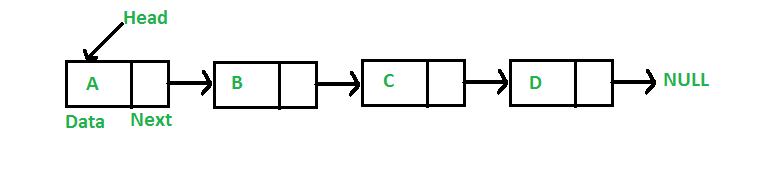
\includegraphics[width=0.9\textwidth]{singly-linked-list.png}
    \caption{Singly Linked List (SLL) \cite{vaghani_2023}}
    \label{fig:singly-linked-list}
\end{figure}
\hfill\medskip\\

\paragraph{Doubly-linked lists (DLL)}
\label{par:doubly-linked-list}
% Doubly-Linked List Definition
\begin{itemize}
    \item \lstinline{DLL} nodes contain three fields: \lstinline{data} field, \lstinline{prev} pointer field and \lstinline{next} pointer field.
    \item Traversal of a \lstinline{DLL} can be done using the \lstinline{next} pointer field or the \lstinline{prev} pointer field. Meaning, the \lstinline{DLL} can be traversed in both directions, from the first node to the last node and vice versa.
    \item The \lstinline{DLL} occupies more memory than a \lstinline{SLL} because it contains a \lstinline{prev} pointer field.
\end{itemize}

% Doubly-Linked List Efficiency Analysis
% \begin{table}[h]
\begin{table}[h]
    \centering
    \caption{Efficiency Analysis of Doubly-Linked List Operations}
    \label{tab:doubly-linked-list-efficiency-analysis}
    \begin{tabular}{|c|c|c|}
        \hline
        Operation           & Worst Case & Average Case \\ \hline
        Access              & $O(n)$     & $O(n)$       \\ \hline
        Search              & $O(n)$     & $O(n)$       \\ \hline
        % Insert              & $O(n)$     & $O(n)$       \\ \hline
        % Delete              & $O(n)$     & $O(n)$       \\ \hline
        Insert (at Head)    & $O(1)$     & $O(1)$       \\ \hline
        Delete (at Head)    & $O(1)$     & $O(1)$       \\ \hline
        Insert (at Current) & $O(1)$     & $O(1)$       \\ \hline
        Delete (at Current) & $O(1)$     & $O(1)$       \\ \hline
        Insert (at Tail)    & $O(1)$     & $O(1)$       \\ \hline
        Delete (at Tail)    & $O(1)$     & $O(1)$       \\ \hline
    \end{tabular}
\end{table}

% Doubly-Linked List Diagram
\begin{figure}[!htbp]
    \centering
    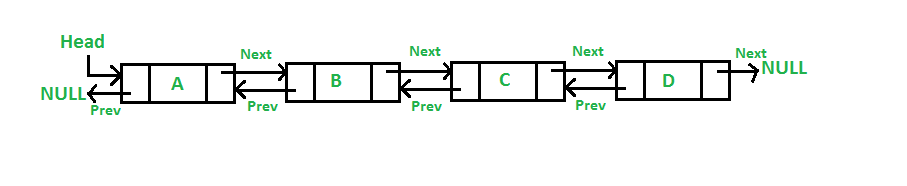
\includegraphics[width=1.1\textwidth]{doubly-linked-list.png}
    \caption{Doubly Linked List (DLL) \cite{vaghani_2023}}
    \label{fig:doubly-linked-list}
\end{figure}
\hfill\medskip\\

% TODO: Check positioning of the figure
\newpage

\paragraph{Advantages}
\begin{itemize}
    \item Efficient insertion and deletion operations at the beginning, end, and middle of the list.
    \item Easy traversal in both directions, allowing for simpler and more flexible algorithms.
    \item Dynamic size, allowing the list to grow and shrink as needed during runtime.
    \item No need for contiguous memory allocation, which allows for better memory utilisation.
    \item Simplified implementation compared to more complex data structures.
\end{itemize}
\paragraph{Disadvantages}
\begin{itemize}
    \item Higher memory overhead due to the storage of two pointers for each node.
    \item Slower random access compared to arrays or hash tables, as elements must be traversed sequentially.
    \item No inherent support for efficient searching, leading to linear search times.
\end{itemize}

\paragraph{Summary}
\hfill\medskip\\
A \lstinline{Doubly Linked List} could be used as the core data structure, but it has some limitations. The sequential nature of the data structure makes it easy to maintain a linear history of changes and revert to previous versions. However, the lack of efficient searching and random access capabilities can slow down operations when dealing with large repositories or complex branching scenarios.

% 
% TODO: Add references
% Advantages and Disadvantages in the context of a Version Control System
% \paragraph{Advantages}
% \begin{itemize}
%     \item Dynamic size: As new versions of a file are created, the \lstinline{Linked List} can grow in size to accommodate the new data, without the need to pre-allocate memory.
%     \item Efficient storage of file changes: Each node in the \lstinline{Linked List} can store the entire contents of a file version, along with metadata such as the date and time the change was made. This allows for efficient storage of file changes over time.
%     \item Easy traversal of file history: The \lstinline{Linked List} structure allows for easy traversal of the file history, as each node contains a reference to the previous version of the file. This makes it easy to track changes and revert to previous versions of a file.
%     \item Memory efficient: The \lstinline{Linked List} structure is memory efficient, as each node only contains the current version of the file and changes made to it, along with simple references to the next and previous nodes in the list. This means that the \lstinline{Linked List} structure does not need to store the entire file history in memory, which can be a significant amount of data.
% \end{itemize}
% \paragraph{Disadvantages}
% \begin{itemize}
%     \item Inefficient retrieval of specific file versions: Retrieving a specific version of a file can be slow, as the \lstinline{Linked List} structure does not allow for random access to the file history. This means that the entire file history must be traversed from the most recent version of the file to the desired version.
%     \item Limited scalability: For large file histories, the \lstinline{Linked List} structure can be less efficient and will not scale as well as other data structures.
%     \item Extra memory overhead: Each node in the \lstinline{Linked List} structure contains a reference to the next and previous nodes in the list, which can add up when dealing with large file histories.
%     \item Not suitable for concurrent access: The \lstinline{Linked List} structure is not suitable for concurrent access, as it is not thread-safe and can lead to data corruption and race conditions.
% \end{itemize}

% % TODO: Add references
% \paragraph{Summary}
% A \lstinline{Doubly-Linked List} is a data structure that consists of a sequence of nodes, each node having a data field and two pointers, one pointing to the next node in the list and the other pointing to the previous node.

% One of the main advantages of using a \lstinline{Doubly-Linked List} is that it allows for easy insertion and deletion of nodes, making it possible to add new file versions or remove outdated ones easily.

% However, Concurrent access to a \lstinline{Doubly-Linked List} can lead to data inconsistencies and race conditions, and proper synchronization must be implemented to prevent these issues.
% \newpage
\subsection{Binary Tree}
% ------------------------------------------------------------------------------
% TODO: Add explanation of why a binary tree is suitable for a Version Control System
% ------------------------------------------------------------------------------
% A \lstinline{Binary Tree} is a hierarchical data structure that consists of a set of nodes, where each node can have at most two children. The topmost node in the tree is called the root node, and the nodes that do not have any children are called leaf nodes. The nodes that have children are called internal nodes. The \lstinline{Binary Tree} structure is a special case of the \lstinline{Tree} data structure, where each node can have at most two children.

A \lstinline{Binary Tree} is a hierarchical data structure in which each node has at most two child nodes, arranged in a way that the value of the node to the left is less than or equal to the parent node and the value of the node to the right is greater than or equal to the parent node. This ordering property ensures efficient search, insertion, and deletion operations. There are several types of binary trees, such as \lstinline{binary search trees}, \lstinline{AVL trees}, and \lstinline{red-black trees}, each with different balancing mechanisms to maintain tree height and performance\cite{mcmahon_2020}.

Each node in a \lstinline{Binary Tree} contains the following elements:
\begin{enumerate}
    \item Data: The data stored in the node.
    \item Left child: A pointer to the left child node.
    \item Right child: A pointer to the right child node.
\end{enumerate}

% % TODO: Add references/Confirm this is correct
% There are several different types of \lstinline{Binary Tree} structures, including:
% \begin{enumerate}
%     \item Full Binary Tree: A \lstinline{Binary Tree} where each node has either zero or two children.
%     \item Complete Binary Tree: A \lstinline{Binary Tree} where all levels of the tree are completely filled, except for the last level. The last level of the tree is filled from left to right.
%     \item Balanced Binary Tree: A \lstinline{Binary Tree} where the difference between the height of the left and right subtrees of any node is not greater than one.
%     \item Degenerate (or Pathological) Binary Tree: A \lstinline{Binary Tree} that is not balanced, where the height of the tree is equal to the number of nodes in the tree.
% \end{enumerate}

% Binary Tree Efficiency Analysis
\begin{table}[h]
    \centering
    \caption{Efficiency Analysis of Binary Tree Operations}
    \label{tab:binary-tree-efficiency-analysis}
    \begin{tabular}{|c|c|c|}
        \hline
        Operation & Worst Case & Average Case \\ \hline
        Search    & $O(n)$     & $O(\log n)$  \\ \hline
        Insert    & $O(n)$     & $O(\log n)$  \\ \hline
        Delete    & $O(n)$     & $O(\log n)$  \\ \hline
    \end{tabular}
\end{table}
% TODO: Add image of binary tree data structure
\begin{figure}[!htbp]
    \centering
    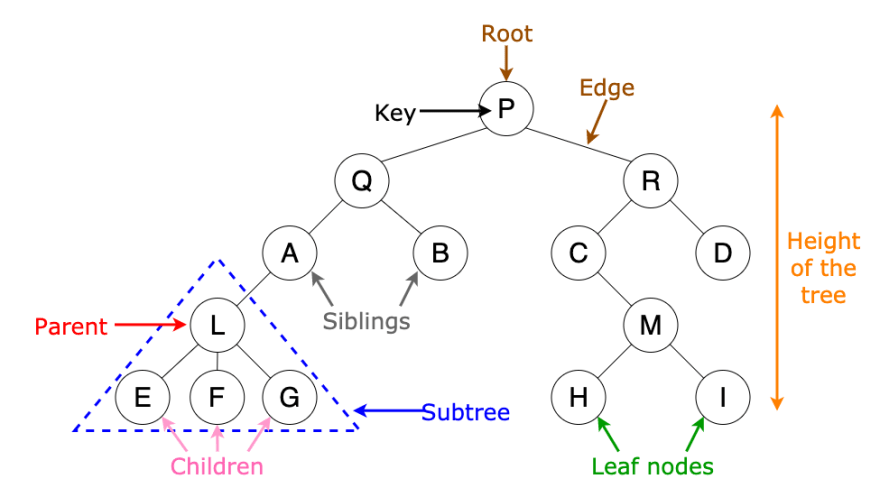
\includegraphics[width=0.8\textwidth]{binary-tree.png}
    \caption{Binary Tree \cite{mcmahon_2020}}
    \label{fig:binary-tree}
\end{figure}
\newpage
% TODO: Add binary tree detailed efficiency analysis of each operation

\paragraph{Advantages}
\begin{itemize}
    \item Efficient search, insertion, and deletion operations when the tree is balanced.
    \item Hierarchical structure allows for natural representation of hierarchical relationships or data with partial order.
    \item Can be easily traversed in various orders (e.g., inorder, preorder, and postorder) to suit different needs.
    \item No need for contiguous memory allocation, which allows for better memory utilisation.
    \item Provides the foundation for more advanced tree structures, like B-trees or trie, that can be used for advanced indexing or searching.
\end{itemize}
\paragraph{Disadvantages}
\begin{itemize}
    \item Unbalanced trees can lead to degraded performance.
    \item Requires more memory overhead compared to linear data structures due to the storage of pointers for each node.
    \item Less suitable for representing non-hierarchical or unordered data.
    \item Can be more complex to implement and maintain compared to simpler data structures.
\end{itemize}

\paragraph{Summary}
\hfill\medskip\\
A \lstinline{Binary Tree} could be used as the core data structure, but it may not be the most suitable choice due to its hierarchical nature. While it can efficiently store and manage version history when dealing with linear or partially ordered data, version control systems often require support for complex branching and merging scenarios, which may not be well-suited for a binary tree.
\smallskip

Additionally, the need for balancing mechanisms to maintain tree height and performance can add complexity to the implementation and maintenance of the system. \lstinline{Directed Acyclic Graphs} or other more advanced data structures might be more appropriate for handling complex functionality.

% % TODO: Add references
% % Advantages and Disadvantages in the context of a Version Control System
% \paragraph{Advantages}
% \begin{itemize}
%     \item Efficient storage of file changes: Each node in the \lstinline{Binary Tree} structure can store the entire contents of a file version, along with metadata such as the date and time the version was created. This allows for efficient storage of file changes, as the entire file history can be stored in a single \lstinline{Binary Tree} structure.
%     \item Easy traversal of file history: The \lstinline{Binary Tree} structure allows for easy traversal of the file history, with the root node representing the most recent version of the file and the leaf nodes representing the oldest versions of the file. This makes it easy to track changes and revert to previous versions of the file.
%     \item Flexibility: \lstinline{Binary Tree} structures can be used to implement a variety of other data structures, such as \lstinline{Binary Search Trees}, \lstinline{AVL Trees}, \lstinline{Heaps}, and others, which can be useful for other operations in a \lstinline{Version Control System}.
% \end{itemize}
% % TODO: Confirm this is correct
% \paragraph{Disadvantages}
% \begin{itemize}
%     \item Inefficient retrieval of specific file versions: The \lstinline{Binary Tree} structure can be slow when retrieving specific file versions, as it requires traversing the \lstinline{Binary Tree} to find the desired node. This can be inefficient when dealing with large file histories.
%     \item Limited scalability: For large file histories, the \lstinline{Binary Tree} structure can be less efficient and may not scale as well as other data structures.
%     \item Extra memory overhead: Each node in the \lstinline{Binary Tree} structure requires extra memory to store the pointers to the left and right child nodes. This can become significant when dealing with large file histories.
%     \item Unbalanced trees can lead to poor performance: If the \lstinline{Binary Tree} structure becomes skewed, the time complexity of searching, insertion, and deletion operations can become \lstinline{O(n)}, where \lstinline{n} is the number of nodes in the tree.
%     \item Not suitable for concurrent access: The \lstinline{Binary Tree} structure is not suitable for concurrent access, as it is not thread-safe. This can lead to data corruption and race conditions.
% \end{itemize}

\subsection{Hash Table}
% ------------------------------------------------------------------------------
% TODO: Add explanation of why a hash table is suitable for a Version Control System
% ------------------------------------------------------------------------------

% A \lstinline{Hash Table} is a data structure that provides an efficient way to store and retrieve key-value pairs. It uses a hash function to map each key to an index in an underlying array, where the corresponding value is stored. When the hash function distributes keys uniformly across the array, hash tables can provide constant-time average-case performance for search, insertion, and deletion operations. In addition, various techniques can be employed to handle collisions (when two keys map to the same index), such as chaining or open addressing.

A \lstinline{Hash Table} is a data structure that uses a hash function to map keys to their corresponding values. It is an efficient way to implement an associative array, where keys are used to look up values.
\smallskip

The basic idea behind a \lstinline{Hash Table} is to use a hash function to map a key to an index in an array, called a bucket, where the corresponding value can be found or stored. The process of mapping a key to an index is called \lstinline{hashing}.
\smallskip

Each element in a \lstinline{Hash Table} consists of:
\begin{enumerate}
    \item Key: This is the value used to look up a corresponding element in the \lstinline{Hash Table}.
    \item Value: This is the value associated with the key that is stored in the \lstinline{Hash Table}.
\end{enumerate}

% TODO: Add references
When a new element is added to a \lstinline{Hash Table}, the key is passed through a \lstinline{hash} function which produces an \lstinline{index} (also called a hash value or bucket) where the element is stored.
When a value is to be retrieved, the key is passed through the same hash function, and the resulting \lstinline{index} is used to look up the corresponding value in the \lstinline{Hash Table}.

% Hash Table Efficiency Analysis
\begin{table}[h]
    \centering
    \caption{Efficiency Analysis of Hash Table Operations}
    \label{tab:hash-table-efficiency-analysis}
    \begin{tabular}{|c|c|c|}
        \hline
        Operation & Worst Case & Average Case \\ \hline
        Search    & $O(n)$     & $\Theta(1)$  \\ \hline
        Insert    & $O(n)$     & $\Theta(1)$  \\ \hline
        Delete    & $O(n)$     & $\Theta(1)$  \\ \hline
    \end{tabular}
\end{table}
% Image of hash table data structure
\begin{figure}[!htbp]
    \centering
    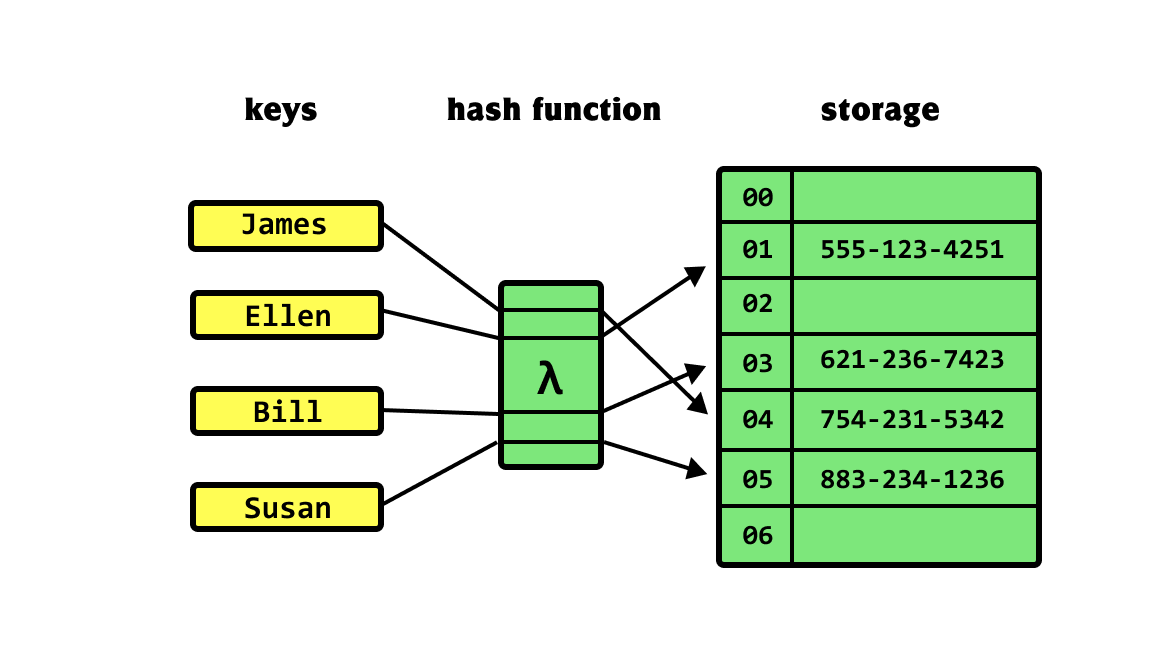
\includegraphics[width=0.8\textwidth]{hash-table.png}
    \caption{Hash Table \cite{stemmler_2022}}
    \label{fig:hash-table}
\end{figure}
\newpage
% TODO: Add hash table detailed efficiency analysis of each operation

\paragraph{Advantages}
\begin{itemize}
    \item Fast average-case performance for search, insertion, and deletion operations.
    \item Supports efficient key-based lookups and direct access to values.
    \item Can be easily resized to accommodate a growing number of key-value pairs, maintaining constant-time complexity.
    \item Suitable for storing unordered or non-hierarchical data.
    \item Provides a foundation for more advanced data structures, like distributed hash tables or bloom filters, used in various applications.
\end{itemize}
\paragraph{Disadvantages}
\begin{itemize}
    \item Requires a good hash function to ensure uniform key distribution and avoid performance degradation due to collisions.
    \item Higher memory overhead compared to linear data structures, as the underlying array needs to be larger than the number of stored key-value pairs to maintain performance.
    \item No inherent support for ordered traversal or range queries, as keys are not stored in a sorted manner.
\end{itemize}

\paragraph{Summary}
\hfill\medskip\\
While \lstinline{Hash Tables} can provide fast and efficient key-based lookups, they may not be the most suitable data structure for the core of a \lstinline{Version Control System}. The lack of inherent support for ordered traversal or range queries can make it difficult to efficiently handle complex branching and merging scenarios that are common in version control systems.
\smallskip

\lstinline{Directed Acyclic Graphs} or other more advanced data structures are often better suited for handling complex branching and merging operations, as they can provide more efficient support for ordered traversal and range queries. Additionally, Version Control Systems typically need to maintain relationships between revisions, which is not a natural fit for the unordered nature of hash tables.
\smallskip

In summary, although \lstinline{Hash Tables} can provide fast key-based lookups and efficient performance in certain scenarios, they may not be the most suitable or scalable choice for the core data structure of a version control system due to their unordered nature and lack of support for ordered traversal or range queries.

% TODO: Add references
% Advantages and Disadvantages in the context of a Version Control System
% \paragraph{Advantages}
% \begin{itemize}
%     \item Efficient searching, insertion, and deletion: A well-implemented \lstinline{Hash Table} allows for these operations to be performed in \lstinline{O(1)} time, which is useful for a Version Control System as it needs to be able to quickly retrieve, insert, and delete file versions.
%     \item Dynamic resizing: \lstinline{Hash Tables} can grow or shrink in size as needed, which is useful for a Version Control System as the number of file versions can vary greatly.
%           % TODO: Confirm that this is true
%     \item Low overhead: A \lstinline{Hash Table} only requires a small amount of overhead for pointers and the hash function, and thus uses less memory than an array or a \lstinline{Linked List} with the same number of elements.
% \end{itemize}
% \paragraph{Disadvantages}
% \begin{itemize}
%     \item{Hash collisions: \lstinline{Hash} functions can produce collisions, where two different keys produce the same \lstinline{index}, leading to the same location in the \lstinline{Hash Table}.}
%     \begin{itemize}
%         \item{\lstinline{Collision resolution techniques}, such as \lstinline{open addressing} and \lstinline{separate chaining}, can be used to handle collisions but it still increases the time complexity of the \lstinline{Hash Table} operations.}
%     \end{itemize}
%     \item Clustering: When all the elements in a \lstinline{Hash Table} are stored in the same bucket, it is called \lstinline{clustering}. This can lead to a performance degradation leading the \lstinline{Hash Table} operations to have the worst-case time complexity of \lstinline{O(n)} for insertion, deletion, and retrieval.
% \end{itemize}

\subsection{Directed Acyclic Graph (DAG)}
% ------------------------------------------------------------------------------
% TODO: Add explanation of why a DAG is suitable for a Version Control System
% ------------------------------------------------------------------------------

A \lstinline{Directed Acyclic Graph (DAG)} is a data structure that consists of nodes connected by directed edges, forming a graph with no cycles. This means that it is impossible to start at a node and follow a sequence of directed edges that leads back to the same node. DAGs are particularly useful for representing dependencies, partial orders, or processes that have a specific sequence of events. For example, in the context of a version control system, a DAG can be used to represent the history of changes made to a project, with nodes representing commits and edges representing parent-child relationships between commits\cite{surti_2016}.

% A \lstinline{Directed Acyclic Graph (DAG)} is a type of graph that consists of a set of nodes and directed edges between pairs of nodes. The edges have direction and they connect one node to another.
% Unlike in a \lstinline{Tree} structure, in a \lstinline{DAG}, a node can have multiple parents and multiple children, but there cannot be any cycles in the graph.

% A node in a \lstinline{DAG} can represent any type of data, and the edges can represent any type of relationship between the nodes. Each node in a \lstinline{DAG} contains the following elements:
% \begin{enumerate}
%     \item Data: The data that the node represents.
%     \item Adjacency list: A list of the nodes that are connected to the current node by an edge.
% \end{enumerate}

% TODO: Add DAG detailed efficiency analysis of each operation
% Directed Acyclic Graph (DAG) Efficiency Analysis
% \begin{table}[h]
%     \centering
%     \caption{Efficiency Analysis of Directed Acyclic Graph (DAG) Operations}
%     % TODO: Create a table of the efficiency analysis of the DAG operations !IMPORTANT!
%     \label{tab:dag-efficiency-analysis}
%     \begin{tabular}{|c|c|c|}
%         \hline
%         Operation & Worst Case & Average Case \\ \hline
%         % Search    & $O(n)$     & $\Theta(1)$  \\ \hline
%         % Insert    & $O(n)$     & $\Theta(1)$  \\ \hline
%         % Delete    & $O(n)$     & $\Theta(1)$  \\ \hline
%     \end{tabular}
% \end{table}
% Image of DAG data structure
\begin{figure}[!htbp]
    \centering
    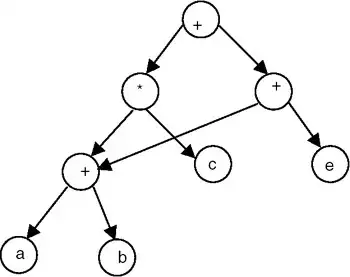
\includegraphics[width=0.5\textwidth]{dag.png}
    \caption{Directed Acyclic Graph (DAG) \cite{surti_2016}}
    \label{fig:dag}
\end{figure}
\newpage

\paragraph{Advantages}
\begin{itemize}
    \item Efficiently represents complex branching and merging scenarios common in Version Control Systems.
    \item Can naturally model dependencies, partial orders, or processes with a specific sequence of events.
    \item Enables efficient algorithms for topological sorting, which can be useful for ordering commits or resolving dependencies.
    \item No need for contiguous memory allocation, which allows for better memory utilisation.
    \item Provides a more expressive and flexible data structure compared to linear or hierarchical structures, making it suitable for various applications.
\end{itemize}
\paragraph{Disadvantages}
\begin{itemize}
    \item Can be more complex to implement and maintain compared to simpler data structures.
    \item Requires more memory overhead compared to linear data structures due to the storage of multiple pointers for each node.
    \item Finding the shortest or most efficient path between nodes can be computationally expensive in large graphs.
    \item No inherent support for fast key-based lookups or direct access to values, as nodes are not indexed by a specific key.
\end{itemize}

\paragraph{Summary}
\hfill\medskip\\
% TODO: Update this summary
\lstinline{Directed Acyclic Graphs} are particularly well-suited for use as the core data structure in a version control system. Their ability to efficiently represent complex branching and merging scenarios allows for more expressive and flexible management of project history. Additionally, the natural modelling of dependencies and partial orders enables efficient algorithms for tasks such as topological sorting and dependency resolution, which are common in version control systems. Overall, the advantages of DAGs in representing complex relationships and dependencies make them a suitable and scalable choice for the core data structure of a version control system.

% % TODO: Add references
% % Advantages and Disadvantages in the context of a Version Control System
% \paragraph{Advantages}
% \begin{itemize}
%     \item Representing complex relationships: \lstinline{DAGs} can be useful for representing complex relationships between different versions of a file, such as \lstinline{branching} and \lstinline{merging} of changes.
%           % TODO: Reconsider this point
%     \item Representing multiple paths: \lstinline{DAGs} can be used to represent multiple paths or multiple possibilities of how a file can change over time.
%           % TODO: Reconsider this point
%     \item Flexibility: \lstinline{DAGs} are very flexible and can be used to represent any type of data and any type of relationship between the data.
% \end{itemize}
% \paragraph{Disadvantages}
% \begin{itemize}
%     \item Complex traversal: Traversing a \lstinline{DAG} can be more complex than traversing a \lstinline{Tree} because there can be multiple paths to traverse, which makes it more difficult to retrieve specific versions of a file.
%     \item Limited scalability: \lstinline{DAGs} may not scale well for large file histories and a large number of versions because they can become very complex and difficult to traverse.
%     \item Not good for searching, insertion, and deletion: \lstinline{DAGs} are not good for searching, insertion, and deletion because they are not ordered and they do not have a root node. This means that the time complexity of these operations is \lstinline{O(n)} due to the need to traverse the entire graph.
% \end{itemize}

% ------------------------------------------------------------------------------

% Algorithms
% ---------------
% What is the essential core functionality of the VCS? (Traversal/Searching, Hashing, Diffing, etc.) - (0.5 page)
% For each functionality, what are the different algorithms that could be used?
% - Explain the algorithms in detail - ((3 x 2) x 1.5 = 9 page)
% - Explain the pros and cons of each algorithm - ((3 x 2) x 0.5 = 3 page)
% - Explain how each algorithm will be implemented - ((3 x 2) x 1 = 6 page)

% What data structures pair well with each algorithm? - (2 page)

% What metrics are important regarding each data structure and algorithm?

% ------------------------------------------------------------------------------

\section{Algorithms}
% \noindent
% TODO: Add intro paragraph


% TODO: Explain the core functionality of the VCS that require algorithms (Traversal/Searching, Hashing, Diffing, etc.)

% ------------------------------------------------------------------------------
\subsection{Searching Algorithms}

\lstinline{Search algorithms} are computational methods to locate specific items, solve problems, or explore and analyse data structures. They are essential tools in computer science, artificial intelligence, and various other domains, as they facilitate efficient processing and management of large datasets. By systematically searching through data or traversing complex structures, these algorithms identify target elements, optimal solutions, or specific patterns.

\subsubsection{Linear Search}
\lstinline{Linear Search} is a simple and straightforward search algorithm that works on unsorted and sorted lists. It sequentially checks each element in the list until the desired element is found or the end of the list is reached \cite{shaalaa_linear_search}. The algorithm compares each element in the list with the target value, starting from the first element and moving through the list one element at a time. Linear Search has an average case time complexity of $O(n)$ and a worst case time complexity of $O(n)$, where $n$ is the number of elements in the list.

% \begin{figure}[htbp]
\begin{figure}[H]
    \centering
    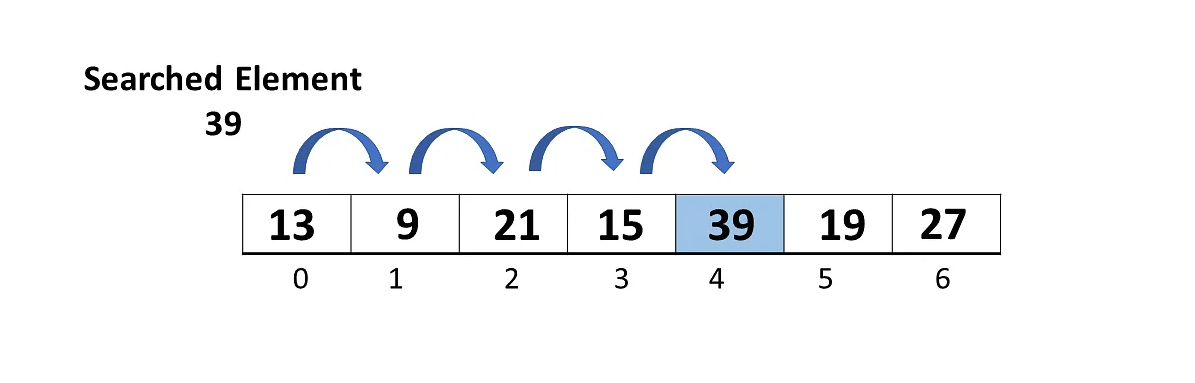
\includegraphics[width=0.8\textwidth]{linear-search-algorithm}
    \caption{Linear Search Algorithm \cite{ravikiran_linear_search}}
    \label{fig:linear-search-algorithm}
\end{figure}

\paragraph{Advantages}
\begin{itemize}
    \item Simple and easy to implement.
    \item Works on unsorted and sorted lists.
    \item No additional memory requirements or data structure modifications needed.
    \item Performs well for small data sets or when the target element is near the beginning of the list.
    \item Can be used as a building block for more advanced search algorithms.
\end{itemize}
\paragraph{Disadvantages}
\begin{itemize}
    \item Inefficient for large data sets, as it has to check each element in the list.
    \item Slower than other search algorithms for sorted lists, such as binary search.
    \item Does not take advantage of any existing order in the list.
    \item May not be suitable for real-time or performance-critical applications.
\end{itemize}

\subsubsection{Binary Search}
\lstinline{Binary Search} is an efficient search algorithm that works on sorted lists \cite{popovi_binary_search}. It repeatedly divides the list in half, comparing the middle element with the target value. If the middle element is equal to the target, the search is successful. If the target value is less than the middle element, the search continues in the left half of the list, otherwise in the right half. This process is repeated until the target value is found or the remaining list becomes empty. Binary Search has an average case time complexity of $O(\log n)$ and a worst case time complexity of $O(\log n)$, where $n$ is the number of elements in the list.

% \begin{figure}[htbp]
\begin{figure}[H]
    \centering
    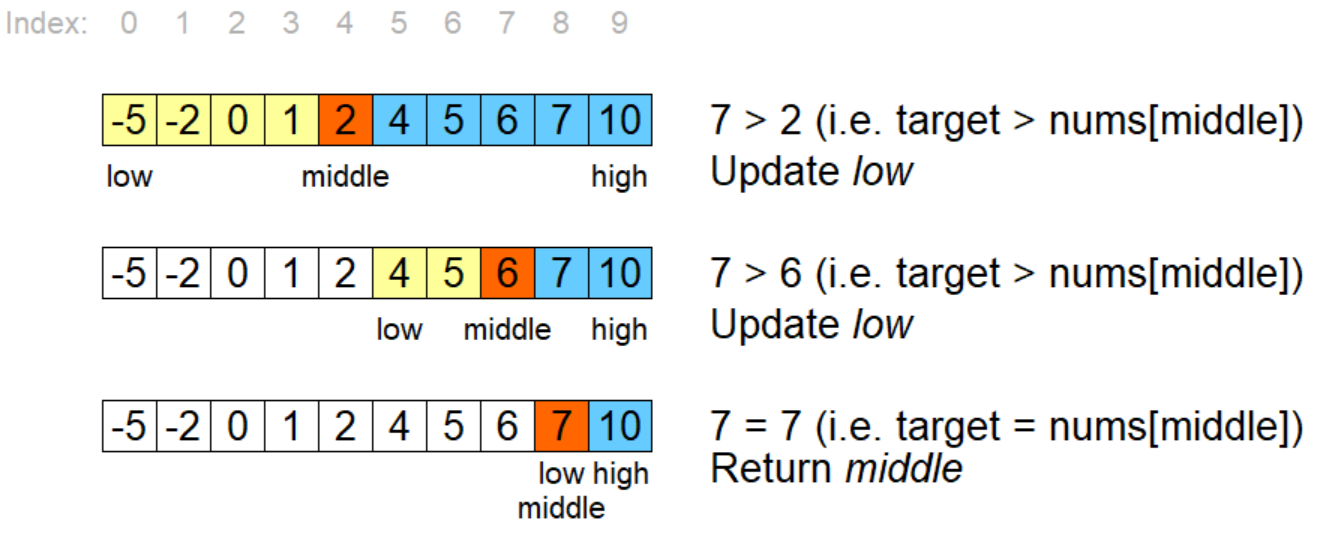
\includegraphics[width=0.8\textwidth]{binary-search-algorithm}
    \caption{Binary Search Algorithm \cite{jamie_binary_search}}
    \label{fig:binary-search-algorithm}
\end{figure}

\paragraph{Advantages}
\begin{itemize}
    \item Efficient search algorithm for sorted lists, with a time complexity of $O(\log n)$.
    \item Takes advantage of the existing order in the list.
    \item Requires fewer comparisons than linear search for large data sets.
    \item Can be implemented iteratively or recursively.
    \item Provides a foundation for more advanced search algorithms, like interpolation search.
\end{itemize}
\paragraph{Disadvantages}
\begin{itemize}
    \item Requires the list to be sorted in ascending order beforehand.
    \item Not suitable for unsorted lists or lists with frequently changing data.
    \item Can be more complex to implement compared to linear search.
    \item Does not work well with large lists stored on slow access media (e.g., hard drives) due to multiple random access operations.
\end{itemize}

\subsubsection{Depth First Search (DFS)}
\lstinline{Depth First Search} is a graph traversal algorithm that explores as far as possible along a branch before backtracking. It can be implemented using recursion or an explicit stack data structure. Starting from a source node, DFS visits a node and marks it as visited. Then, it recursively explores each unvisited neighbour of the current node, treating the neighbor as the new current node. The algorithm continues this process until all reachable nodes have been visited. DFS has an average case time complexity of $O(V + E)$ and a worst case time complexity of $O(V + E)$, where $V$ is the number of vertices and $E$ is the number of edges in the graph.

% \begin{figure}[htbp]
\begin{figure}[H]
    \centering
    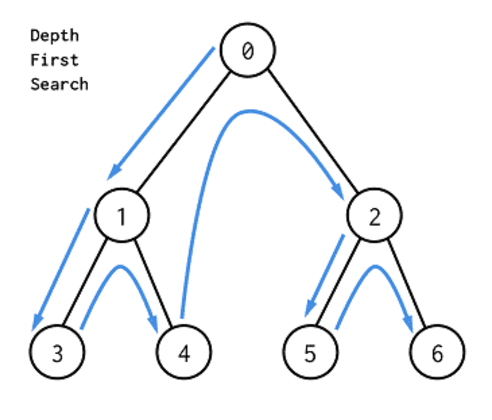
\includegraphics[width=0.5\textwidth]{depth-first-search-algorithm}
    \caption{Depth First Search Algorithm \cite{zaltsman_dfs_bfs}}
    \label{fig:depth-first-search-algorithm}
\end{figure}

\paragraph{Advantages}
\begin{itemize}
    \item Can be used to find connected components, cycles, and paths in a graph.
    \item Effective for searching large, sparsely connected graphs.
    \item Can be implemented using recursion or an explicit stack data structure.
    \item Visits nodes in a linear and natural order.
    \item Can be adapted for other graph traversal problems, like topological sorting.
\end{itemize}
\paragraph{Disadvantages}
\begin{itemize}
    \item May consume a large amount of memory for deep graphs when implemented recursively.
    \item Can get stuck in cycles if not properly implemented with visited node tracking.
    \item Does not always find the shortest path in weighted graphs.
    \item May be less intuitive than Breadth First Search for certain problems.
\end{itemize}

\subsubsection{Breadth First Search (BFS)}
\lstinline{Breadth First Search} is a graph traversal algorithm that visits all nodes at the same level before moving on to the next level. It can be implemented using a queue data structure. Starting from a source node, BFS visits and marks the node as visited. Then, it enqueues all unvisited neighbors of the current node. Finally, the algorithm dequeues the next node from the front of the queue and repeats the process until the queue is empty, ensuring that all reachable nodes have been visited. BFS has an average case time complexity of $O(V + E)$ and a worst case time complexity of $O(V + E)$, where $V$ is the number of vertices and $E$ is the number of edges in the graph.

% TODO: Check placement of figure
% \newpage
\begin{figure}[htbp]
    \centering
    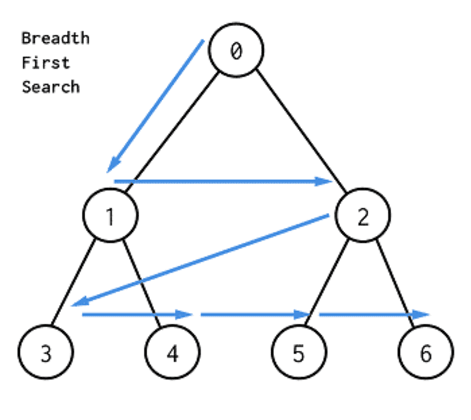
\includegraphics[width=0.5\textwidth]{breadth-first-search-algorithm}
    \caption{Breadth First Search Algorithm \cite{zaltsman_dfs_bfs}}
    \label{fig:breadth-first-search-algorithm}
\end{figure}
% \hfill\medskip\\
% \newpage

\paragraph{Advantages}
\begin{itemize}
    \item Can be used to find the shortest path in unweighted graphs or determine the level of each node from the source node.
    \item Effective for searching large, densely connected graphs.
    \item Can be implemented using a queue data structure, avoiding recursion.
    \item Visits nodes in a level-wise order, which can be more intuitive for certain problems.
    \item Can be adapted for other graph traversal problems, like bipartite graph checking.
\end{itemize}
\paragraph{Disadvantages}
\begin{itemize}
    \item Can consume a large amount of memory for densely connected graphs due to the use of a queue.
    \item Not well-suited for finding all paths or connected components in a graph.
    \item Does not work efficiently for searching large, sparsely connected graphs.
    \item Can be slower than \lstinline{Depth First Search} for certain problems, such as finding cycles or connected components.
\end{itemize}

% ------------------------------------------------------------------------------

\subsection{Diffing Algorithms}

\lstinline{Diffing algorithms}, also known as difference algorithms or delta algorithms, are specialised computational methods designed to identify and highlight the differences between two sets of data. These algorithms compare input sequences, such as text, code, or binary data, to efficiently determine the changes needed to transform one sequence into the other. By detecting additions, deletions, and modifications, diffing algorithms enable the tracking and management of revisions in a concise and comprehensible manner.

\subsubsection{Myers Diff Algorithm}
The \lstinline{Myers diffing algorithm}, developed by Eugene W. Myers, is an efficient algorithm for comparing two sequences (such as lines in text files) and finding the shortest edit script that transforms one sequence into the other. The algorithm is based on the concept of an edit graph, where each node represents an element in the sequences, and the edges represent insertions, deletions, or matches. The algorithm finds the shortest path through this graph, also known as the \lstinline{Longest Common Subsequence (LCS)} path, which represents the minimal set of edits required to transform one sequence into the other\cite{coglan_myers_2017}.
\smallskip

The time and space complexity of the \lstinline{Myers Diff} algorithm is $O(ND)$, where $N$ is the sum of the lengths of both inputs, and $D$ is the size of the minimum edit script that converts one input to the other. When the number of differences is small, various optimisations can be applied to improve complexity up to $O(N\log N + D^2)$ time and $O(N)$ space.

% TODO: Add diagram for Myers diff algorithm

\paragraph{Advantages}
\begin{itemize}
    \item Efficiently finds the shortest edit script, reducing the number of changes needed to transform one sequence into the other.
    \item Can handle large input sequences, as it has a linear space complexity.
    \item Can be adapted for various applications, such as comparing text files, source code, or DNA sequences\cite{coglan_myers_2017}.
    \item The algorithm is well-established and widely used, making it a reliable choice for many diffing tasks.
\end{itemize}
\paragraph{Disadvantages}
\begin{itemize}
    \item Can produce suboptimal diffs for specific cases, such as when comparing sequences with many common elements but in a different order.
    \item The algorithm's implementation can be complex and difficult to understand for those unfamiliar with graph-based algorithms.
    \item May not be the most efficient algorithm for all diffing tasks, as other algorithms may produce better results in specific cases.
    \item The quality of the output can be sensitive to the choice of the underlying \lstinline{Longest Common Subsequence} algorithm.
\end{itemize}

\subsubsection{Patience Diff Algorithm}
The \lstinline{Patience Diffing algorithm}, developed by Bram Cohen, is a diffing algorithm that aims to produce more human-readable diffs by focusing on finding the \lstinline{Longest Common Subsequence (LCS)} in the two sequences. The algorithm first identifies unique matching lines (or elements) between the sequences and sorts them by their position in the first sequence. Then, it finds the \lstinline{LCS} in the sorted list of positions from the second sequence. The algorithm recursively applies this process to the unmatched portions of the sequences until the entire diff is produced\cite{coglan_patience_2017}.
\smallskip

The time complexity of the \lstinline{Patience Diff} algorithm is $O(N\log N)$, where $N$ is the sum of the lengths of both inputs.

% TODO: Add diagram for Patience diff algorithm

\paragraph{Advantages}
\begin{itemize}
    \item Produces more human-readable diffs, as it focuses on preserving the order of common elements.
    \item Can handle large input sequences, as it has a linearithmic time complexity\cite{coglan_patience_2017}.
    \item Can be used as a standalone algorithm or in combination with other diffing algorithms, such as the Myers algorithm, to improve the quality of the output.
    \item The algorithm is relatively simple and straightforward to implement compared to some other diffing algorithms.
    \item Works well for cases where the sequences have many common elements but in a different order.
\end{itemize}
\paragraph{Disadvantages}
\begin{itemize}
    \item May produce suboptimal diffs for specific cases, such as when comparing sequences with many non-unique elements.
    \item The algorithm's performance depends on the choice of the underlying \lstinline{LCS} algorithm.
    \item May not be the most efficient algorithm for all diffing tasks, as other algorithms may produce better results in specific cases.
    \item Not as widely used or well-established as some other diffing algorithms, such as the \lstinline{Myers algorithm}.
\end{itemize}

% ------------------------------------------------------------------------------